% $Header$

\documentclass{beamer}
\usefonttheme[onlymath]{serif}
\newcommand\bmale{\fontsize{6}{7.2}\selectfont}
\newcommand\male{\fontsize{8}{7.2}\selectfont}
\newcommand\normalne{\fontsize{10}{7.2}\selectfont}
\newcommand\duze{\fontsize{12}{7.2}\selectfont}
\setbeamertemplate{caption}{\raggedright\insertcaption\par}
% This file is a solution template for:

% - Talk at a conference/colloquium.
% - Talk length is about 20min.
% - Style is ornate.



% Copyright 2004 by Till Tantau <tantau@users.sourceforge.net>.
%
% In principle, this file can be redistributed and/or modified under
% the terms of the GNU Public License, version 2.
%
% However, this file is supposed to be a template to be modified
% for your own needs. For this reason, if you use this file as a
% template and not specifically distribute it as part of a another
% package/program, I grant the extra permission to freely copy and
% modify this file as you see fit and even to delete this copyright
% notice. 


\mode<presentation>
{
  \usetheme{CambridgeUS}
  \usecolortheme{beaver}
  % or ...

  %\setbeamercovered{transparent}
  % or whatever (possibly just delete it)
}

\usepackage{ulem}
\usepackage{tabto}
\usepackage[]{algorithm2e}
\usepackage{bm}
\usepackage{lmodern}
\usepackage[T1]{fontenc}
\usepackage[polish]{babel}
\usepackage[utf8]{inputenc}
\DeclareMathOperator*{\argmin}{argmin}
\DeclareMathOperator*{\argmax}{argmax}
\selectlanguage{polish}
% or whatever

%\usepackage[latin1]{inputenc}
%% or whatever

% Or whatever. Note that the encoding and the font should match. If T1
% does not look nice, try deleting the line with the fontenc.


\title[Analizy mikrosymulacyjne] % (optional, use only with long paper titles)
{Analizy mikrosymulacyjne - wykłady}

\subtitle
{Symulacja systemu komunikacji zbiorowej}

\author[dr inż. Rafał Kucharski] % (optional, use only with lots of authors)
{dr inż. Rafał~Kucharski\inst{1}}
% - Give the names in the same order as the appear in the paper.
% - Use the \inst{?} command only if the authors have different
%   affiliation.

\institute[] % (optional, but mostly needed)
{
  \inst{1}%
  Zakład Systemów Komunikacyjnych\\
  Politechnika Krakowska
  \and
 }
% - Use the \inst command only if there are several affiliations.
% - Keep it simple, no one is interested in your street address.

\date[ZSK, L-2, WIL, PK] % (optional, should be abbreviation of conference name)
{Kraków, 2017}
% - Either use conference name or its abbreviation.
% - Not really informative to the audience, more for people (including
%   yourself) who are reading the slides online



% If you have a file called "university-logo-filename.xxx", where xxx
% is a graphic format that can be processed by latex or pdflatex,
% resp., then you can add a logo as follows:

\pgfdeclareimage[height=1cm]{university-logo}{ZSK}
 \logo{\pgfuseimage{university-logo}}

% Delete this, if you do not want the table of contents to pop up at
% the beginning of each subsection:
\AtBeginSubsection[]
%{
%  \begin{frame}<beamer>{Outline}
%    \tableofcontents[currentsection,currentsubsection]
%  \end{frame}
%}


% If you wish to uncover everything in a step-wise fashion, uncomment
% the following command: 

%\beamerdefaultoverlayspecification{<+->}


\begin{document}

\begin{frame}
  \titlepage
\end{frame}

%\begin{frame}{Zakres}
%  \tableofcontents
%  % You might wish to add the option [pausesections]
%\end{frame}


% Structuring a talk is a difficult task and the following structure
% may not be suitable. Here are some rules that apply for this
% solution: 

% - Exactly two or three sections (other than the summary).
% - At *most* three subsections per section.
% - Talk about 30s to 2min per frame. So there should be between about
%   15 and 30 frames, all told.

% - A conference audience is likely to know very little of what you
%   are going to talk about. So *simplify*!
% - In a 20min talk, getting the main ideas across is hard
%   enough. Leave out details, even if it means being less precise than
%   you think necessary.
% - If you omit details that are vital to the proof/implementation,
%   just say so once. Everybody will be happy with that.
\section{Wykład 2: Symulacja systemu komunikacji zbiorowej}
\subsection{Wstęp}

\begin{frame}{Wstęp}{symulacja komunikacji zbiorowej}

\alert{komunikacja zbiorowa} to dwa osobne systemy, które symulujemy osobno:
\begin{description}
\item[pojazdy] autobusy, pociągi kursujące po zadanych trasach z zadanym rozkładem
\item[pasażerowie] korzystający z komunikacji zbiorowej żeby dotrzeć do celu.
\end{description}

\end{frame}

\subsection{Sieć}
\begin{frame}{Sieć}{rozkład jazdy}
znacznie bardziej złożony niż graf sieci transportowej. Wiele formatów, np. VDV, HAFAS, GTFS, ...\\
\begin{center}
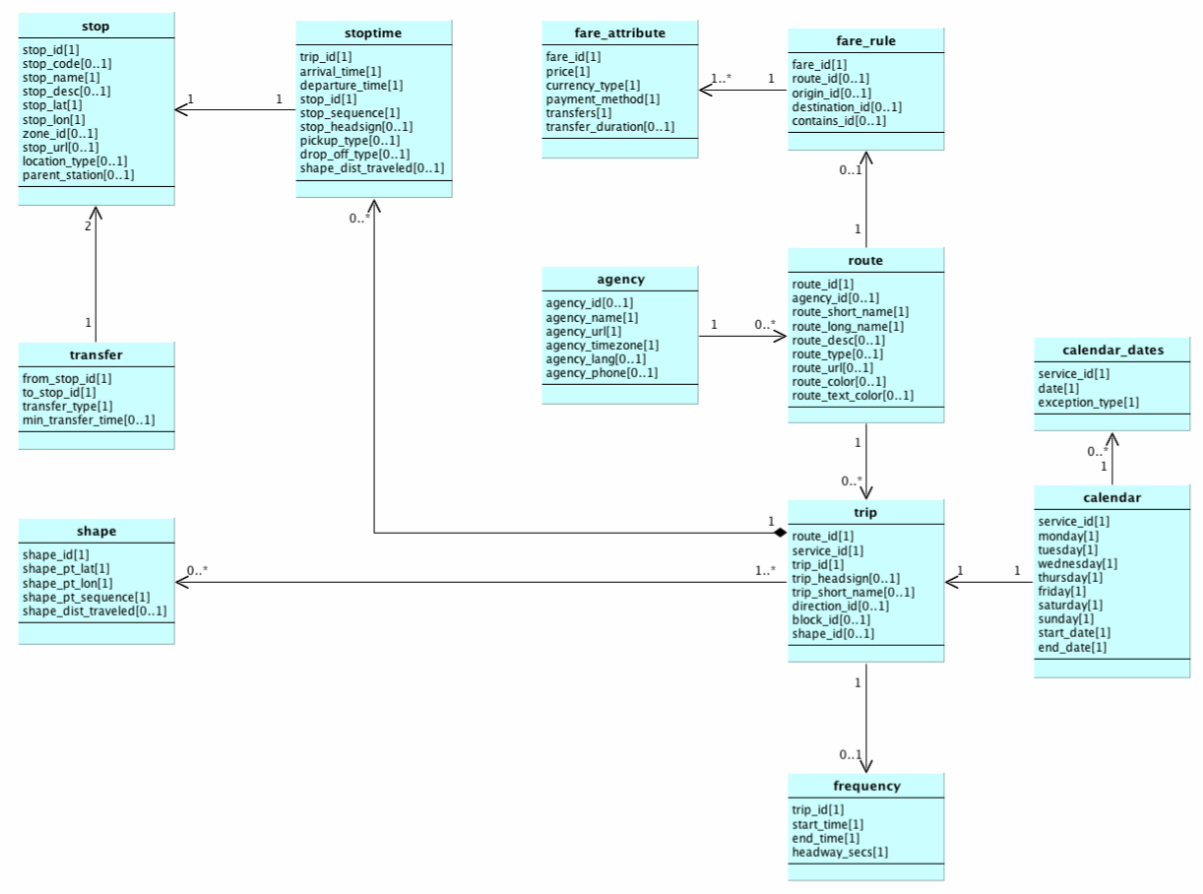
\includegraphics[scale=0.2]{gtfs}
\end{center}
\end{frame}

\begin{frame}{Sieć}{graf diachroniczny}
\begin{center}
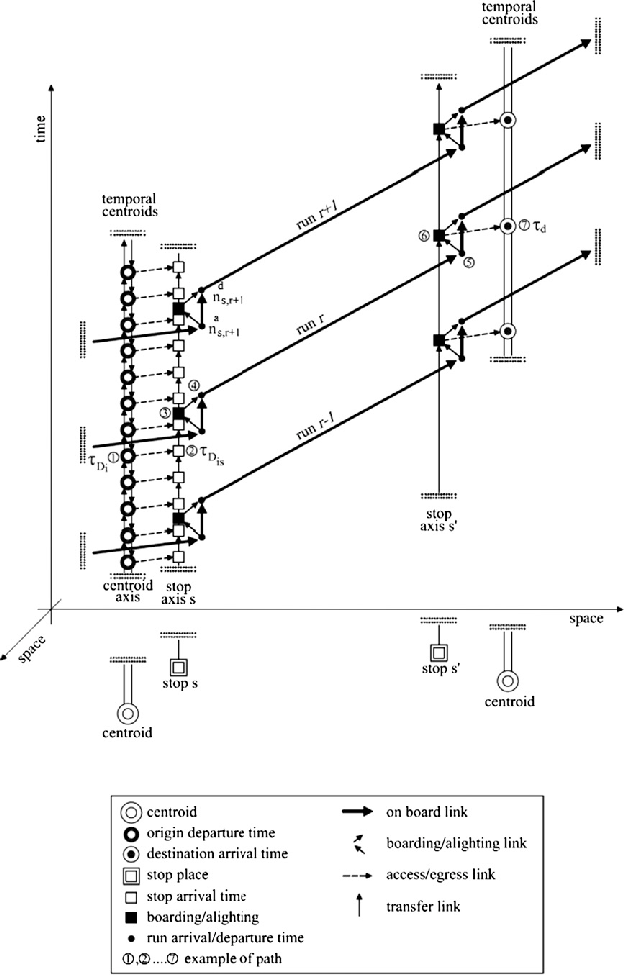
\includegraphics[scale=0.5]{diachronic}
\end{center}
\end{frame}
%
\begin{frame}{Sieć}{Przykład sieci}
\begin{center}
\includegraphics[scale=0.5]{piesflorian}
\end{center}
\end{frame}
%
\begin{frame}{Sieć}{Model przystanku}
\includegraphics[scale=0.455]{stopmodel}
\end{frame}

\subsection{Symulacje}
\begin{frame}{Symulacje}{Symulator komunikacji zbiorowej}
\alert{BusMezzo} mezoskopowe \alert{???} otwarte środowisko do symulacji (C++). \\ Działa dla dowolnej sieci, importer z i do Visuma (w produkcji w ZSK), rozkład jazdy lub model interwałowy. 
\end{frame}

\begin{frame}{Symulacje}{Przepływ pojazdów}
\alert{BusMezzo} dla zadanych odjazdów z przystanków początkowych symuluje przejazd pojazdów przez sieć, uwzględniając wpływ ruchu drogowego i procesu wymiany na czas przejazdu.
\end{frame}

\begin{frame}{Symulacje}{Przepływ pojazdów}
\begin{center}
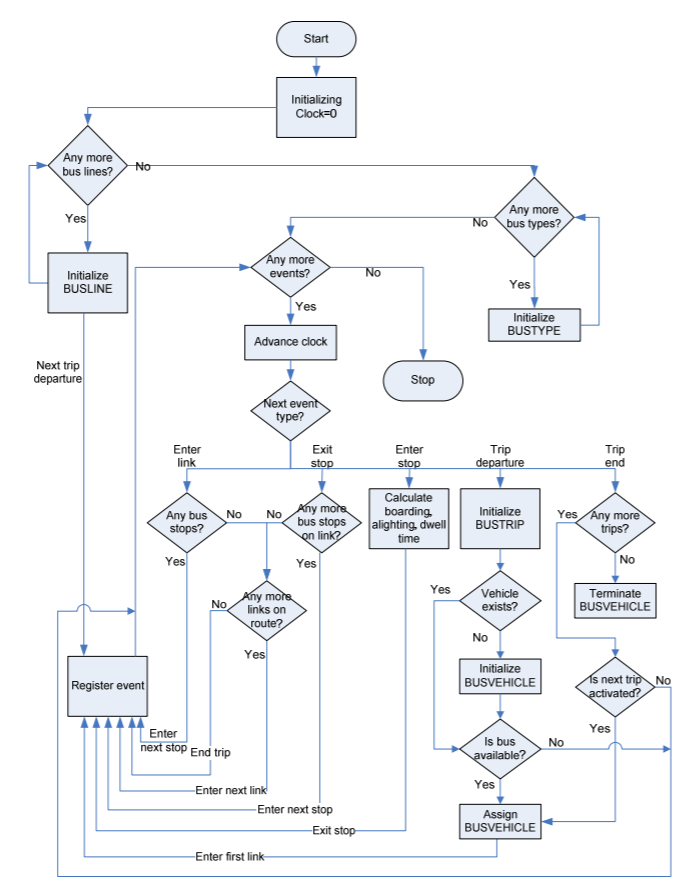
\includegraphics[scale=0.4]{Cats1}
\end{center}
\end{frame}

\begin{frame}{Symulacje}{Przepływ pojazdów}
\begin{center}
Czas wymiany jako funkcja:
\begin{enumerate}
\item liczby wsiadających
\item liczby wysiadających
\item zapełnienia
\item szerokości i liczby drzwi
\item organizacji (wsiadanie przodem, najpierw wsiadamy potem wysiadamy, płatność przy wejściu, odbicie biletu, itp.)
\end{enumerate}
\end{center}
\end{frame}

\begin{frame}{Symulacje}{Przepływ pasażerów}
Podróżni w \alert{BusMezzo} dokonują wyborów:
dokonują oni wyborów:
\begin{itemize}
\item jaki przystanek początkowy. (decyzja przy źródle) \\ \includegraphics[scale=0.1]{sr}
\item którą linię wybiorą na przystanku.\\ \includegraphics[scale=0.1]{stopmodel}
\item na którym przystanku wysiądą.
\item do której linii się przesiądą.
\end{itemize}
\end{frame}

\begin{frame}{Symulacje}{Przepływ pasażerów}
\begin{center}
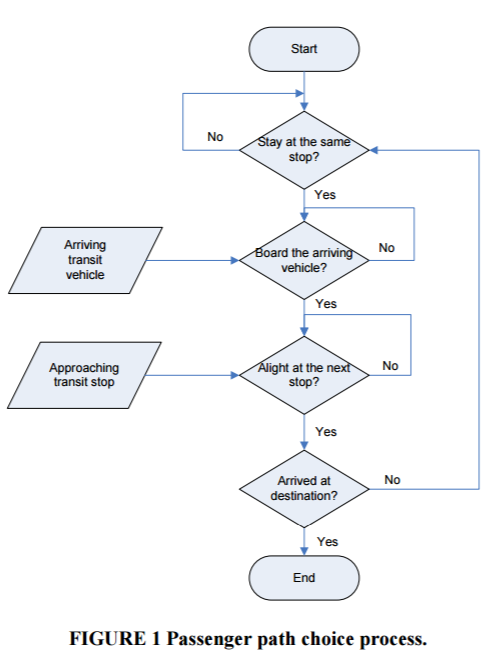
\includegraphics[scale=0.455]{Pass}
\end{center}
\end{frame}

\begin{frame}{Symulacje}{Przepływ pasażerów}
\male
Większość decyzji upraszczana jest do binarnego modelu logitowego \\
 \begin{itemize}
\item wsiadam - nie wsiadam i czekam dalej
\item wysiadam - zostaję i jadę dalej
\end{itemize}
dodatkowo model wyboru ścieżki w sieci pieszej (w ramach przesiadki, lub poszukiwania przystanku początkowego/końcowego)
\begin{equation*}
P_{board} = \frac{e^{\mu \cdot V_{board}}}{e^{\mu \cdot V_{board}} + e^{\mu \cdot V_{stay}}}
\end{equation*}
\male
określ użyteczność $V$ aktualnie przyjeżdżającej linii (czas dojazdu, koszt, komfort, liczba przesiadek, czas dojścia itp.) i porównaj z kosztami linii które dojeżdżają później (\textit{logsum}):
\begin{equation*}
V_{stay} = ln \sum_{r' \in R^+} e^{\mu \cdot V_{r'}}
\end{equation*}
model probabilistyczny: $V=U+ \varepsilon$ (błąd  $\varepsilon = Logistic(0,\mu)$).
\end{frame}


\begin{frame}{Symulacje}{Wyniki BM}
\begin{center}
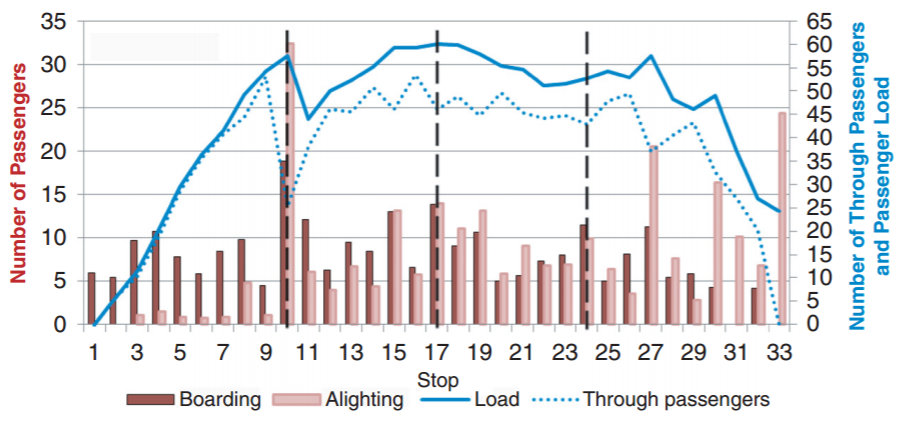
\includegraphics[scale=0.455]{BM}
\end{center}
\end{frame}

\subsection{Zagadnienia egzaminacyjne}
\begin{frame}{Zagadnienia}{pytania egzaminacyjne}
\end{frame}

\begin{frame}{Zagadnienia}{Wykład 1}
\bmale
\begin{enumerate}
\item Czym różnią się deterministyczny i niedeterministyczny opis ruchu, jakie są wady i zalety każdego z nich?
\item Opisz czym różnią się modele makroskopowe od mikroskopowych i statyczne od dynamicznych?
\item Jakie parametry ruchu możemy odczytać z zapisuje trajektorii pojazdów w ujęciu droga-czas?
\item Naszkicuj zakładana w diagramie fundamentalnym zależność pomiędzy: 
\begin{itemize}
\bmale
\item gęstością, a potokiem
\item prędkością a potokiem 
\item gęstością, a prędkością
\end{itemize}
\item Dla zadanego wykresu droga czas z naniesionymi trajektoriami:
\begin{itemize}
\bmale
\item jaki jest czas przejazdu i opóźnienie dla pogrubionego pojazdu?
\item jaki jest dopływ pojazdów/h dla t<20 (poj./h)?
\item jaka jest prędkość w ruchu swobodnym (km/h)?
\item jaka jest gęstość pojazdów w kolejce (poj./km)?
\item jaka jest gęstość odpływu po usunięciu przeszkody (poj./h)?
\item jaka jest prędkość fal: budowania i rozładowywania się kolejki (km/h)?
\end{itemize}
\end{enumerate}
\end{frame}

\begin{frame}{Zagadnienia}{Wykład 2}
\bmale
\begin{enumerate}
\item Opisz różnicę pomiędzy mikrosymulacją a algorytmem rozkładu ruchu na sieć i opisz miejsce mikrosymulacji w modelu czterostadiowym.
\item Podaj opis stanu pojazdu w modelu mikroskopowym.
\item Podaj i omów algorytm mikrosymulacji ruchu.
\item Opisz podstawowe decyzje kierowcy w ujęciu mikroskopowym: ciągłe i dyskretne, oraz opis stanu jaki potrzebny jest do ich symulacji.
\item Omów trajektorię zbliżania się pojazdów w modelu Wiedemanna.
\item Czym różni się optymalny przejazd pojazdu przez sieć drogową od przejazdu kierowcy w modelu mikrosymulacyjnym
\item Opisz wyniki mikrosymulacji, oraz sposób pracy z nimi. Jak można je interpretować. Ile symulacji powinno się wykonać, żeby zyskać pewność.
\item Podaj przykładową miarę dopasowania modelu mikrosymulacji, oraz przykładowy sposób jego kalibracji.
\item Jak możemy odwzorować sygnalizacje świetlną w modelu, oraz jak można wykorzystać model symulacyjny przy projektowaniu systemów sterowania ruchem
\item Jak generowane są pojazdy w modelu mikroskopowym? Jaka uwzględniana jest losowość dopływu? Jak uzyskać rzeczywistą strukturę potoku na granicy modelu?
\end{enumerate}
\end{frame}



\subsection{Podsumowanie}
\begin{frame}{Dziękuję za uwagę}{zapraszam do dyskusji}
\bmale źródła wszystkich obrazów (jeśli nie podano inaczej) \\ G. Gentile, K. Noekel eds., Modelling Public Transport Passenger Flows in the Era of Intelligent Transport Systems Springer 2016, lub własne
\end{frame}



\end{document}
